\documentclass[12pt]{article}
 
%\usepackage{fullpage}
\usepackage{hyperref}
\usepackage{color}
\usepackage{colortbl}
\usepackage{graphicx}
\DeclareGraphicsExtensions{.pdf,.png,.gif,.jpg}
%\usepackage{tabular}
  
\title{A Study to Enhance the Sensitivity for the Discovery of the Higgs Boson Coupling to Dimuons}
\author{Brendan Regnery, Darin Acosta, Justin Hugon}
\date{\today}
\begin{document}
\maketitle
 
\section{Introduction}

The smallest Higgs coupling directly observable at the LHC is $H\rightarrow \mu \mu$. 
An analysis, looking for this channel, has already been run on data received from the 8 TeV run of the LHC. 
This analysis reported an observed limit of 12 times the standard model \cite{hmumuPap} 
we hope to improve upon this analysis for the next run of the LHC at 13 TeV \cite{AN2012_459}. 

The current analysis optimized a category for the Vector Boson Fusion (VBF) channel and included, 
but did not optimize, an associated production with a vector boson channel (VH). 
In order to improve upon this analysis, we looked into optimizing the VH channel (where $H\rightarrow \mu \mu$ and $V\rightarrow jj$) for 8 TeV data, 
altering the background fit in the current analysis, and creating an analysis with these changes to run on simulated 13 TeV data.

\section{Data Samples}

Our first analysis uses simulated data. These are the methods that we used to obtain our simulated data.

\subsection{Simulated Signal Samples}

Our Gluon-fusion and VBF signal samples were produced using the \textsc{powheg-box} NLO generator~\cite{powheg1,powheg2,powheg3} 
interfaced with \textsc{pythia} 6~\cite{pythia} for parton showering.
For the associated production samples, we used the \textsc{herwig}++ event generator and 
parton shower program~\cite{herwigpp}.  NLO corrections are calculated using the 
POWHEG implementation built into \textsc{herwig}++. 
In our associated production samples, the W or Z bosons were allowed to decay without restriction.
Each signal sample contains 100k events.

For gluon-fusion, VBF, and associated production, we used samples with $m_H =$ 125~$\textrm{GeV}/\textrm{c}^{2}$. 
The names of the datasets are shown in Table \ref{tab:sigDatasets}

\begin{table}[htb]
\caption{Simulated signal dataset names used in the analysis.
\label{tab:sigDatasets}
}
\small
\begin{center}
\begin{tabular}{ |p{12cm}|}
\hline
Signal Dataset Name \\
\hline
\hline
/GluGlu\_HToMM\_M-125\_TuneZ2star\_8TeV-powheg-pythia6/Summer12\_DR53X-PU\_S10\_START53\_V7C-v1/AODSIM \\
\hline
/VBF\_HToMM\_M-125\_TuneZ2star\_8TeV-powheg-pythia6/Summer12\_DR53X-PU\_S10\_START53\_V7C-v1/AODSIM \\
\hline
/WH\_HToMuMu\_M-125\_8TeV-powheg-herwigpp/Summer12\_DR53X-PU\_S10\_START53\_V19-v1/AODSIM \\
\hline
/ZH\_HToMuMu\_M-125\_8TeV-powheg-herwigpp/Summer12\_DR53X-PU\_S10\_START53\_V19-v1/AODSIM \\
\hline
\end{tabular}
\end{center}
\end{table}

% End Signal Samples
%%%%%%%%%%%%%%%%%%%%%%%%%%%%%%%%%%%%%%%%%%%%%%%%%%%%%%%%%%%%%%%%%%%%%%
% Begin Background Samples

\subsection{Simulated Background Samples}

The simulated background samples used in our analysis are listed in 
Table~\ref{tab:BGSamples8TeV}.

\begin{table}[h]
\begin{center}
\caption{\label{tab:BGSamples8TeV} Background MC samples at $\sqrt{s}=8$ TeV}
\begin{tabular}{|p{10cm}|c|c|c|c|} \hline
Sample & Original  & $\sigma$ [pb] & Equivalent \\
 &  \# Events &  &  Lumi [1/$fb$] \\
\hline
\hline
/DYJetsToLL\_M-50\_TuneZ2Star\_8TeV-madgraph-tarball/Summer12\_DR53X-PU\_S10\_START53\_V7A-v1/AODSIM &	     30086987 &	  3503.71 &   8.6  \\
\hline                                                                                                                                     
/TTJets\_MassiveBinDECAY\_TuneZ2star\_8TeV-madgraph-tauola/Summer12\_DR53X-PU\_S10\_START53\_V7A-v3/AODSIM &  6921652 &	  225.197 &  30.7  \\
\hline                                                                                                                                                       /WW\_TuneZ2star\_8TeV\_pythia6\_tauola/Summer12\_DR53X-PU\_S10\_START53\_V7A-v1/AODSIM & 	              5218045 &	   54.838 &  95.2  \\
\hline                                                                                                                                     
/WZ\_TuneZ2star\_8TeV\_pythia6\_tauola/Summer12\_DR53X-PU\_S10\_START53\_V7A-v1/AODSIM &	             10000283 &	    33.21 & 301    \\
\hline                                                                                                                                     
/ZZ\_TuneZ2star\_8TeV\_pythia6\_tauola/Summer12\_DR53X-PU\_S10\_START53\_V7A-v1/AODSIM 	&  	              9799908 &    17.654 & 555	   \\
\hline
\end{tabular}
\end{center}
\end{table}

\section{Muon and Jet Object Definitions}

In our analysis on simulated data, events are required to pass a simulated \texttt{HLT\_IsoMu24\_eta2p1} trigger.
In all of our analyses, events are also required to contain a pair of opposite-sign muons with $|\eta|<2.1$.
A muon must be matched to the trigger (within $\Delta R = \sqrt{(\Delta \phi)^2+(\Delta \eta)^2}< 0.2$), 
and have $p_T>25$\,GeV, while the other muon must have $p_T>15$\,GeV.
Both muons must pass the ``tight'' muon ID requirements~\cite{AN2012_459}.
as well as being isolated from other event activity.  We quantified Isolation using
particle-flow (PF) relative isolation corrected for pileup using the ``$\delta \beta$''
procedure~\cite{AN2012_459}.  Each muon is required to have a PF relative isolation value
of less than 0.12.  Additionally, the 3D opening angle between the two muons must be
smaller than $\pi-0.02$ radians, and events must contain a well reconstructed primary
vertex.
In the case where there are more than two muons in an event, all pairs passing the above
requirements are considered, and will be referred to as separate events for the remainder
of this note.  

The simulated muon selection efficiency is corrected to match the data using 
the ``tag-and-probe'' method, using scale factors.  The muon momentum resolution
is also corrected to match the resolution of the MuScleFit-corrected data~\cite{AN2012_459}.

Jets are reconstructed from PF candidates clustered with the anti-$k_t$ algorithm with
a radius parameter of 0.5.  The $p_T$ and $|\eta|$ requirements of the jets are varied in
the below optimization.  A loose jet ID is applied~\cite{AN2012_459}, and a further
MVA-based selection is applied to reject jets formed from pileup particles~\cite{PUID}.

\section{VH Selection Criteria}

\subsection{Introduction}

We began improving the $H \rightarrow \mu \mu$ analysis by creating and optimizing additional selection criteria in the VH category. 
Since all of categories in the current analysis were looking at $H \rightarrow \mu \mu$, we kept the same dimuon 
selection for VH (as specified in the Muon Object Definitions). 
The current analysis selected jets with $p_{T}, \eta,$ and mass values expected in the VBF channel, but in VH the jets originated from the vector boson. 
Therefore we altered the jet selection criteria in the VH category to specifically look for $V \rightarrow jj$.

The biggest background contributors in the VH channel are Drell Yan ($DY$) and top quark decays ($t\overline{t}$), 
so our ultimate goal, with the jet selection, is to optimize the VH signal over these two background contributors.

\subsection{Basic Jet Selection Criteria}

In the VBF channel, jets are predicted to have a high $p_{T}$ and a more forward position in the detector (i.e. high $\eta$). 
Comparatively, jets in the VH channel are predicted to have a lower $p_{T}$ and a lower $\eta$. 
Therefore, we decided to investigate lowering our $p_{t}$ and $\eta$ criteria.

\subsection{Dijet Invariant Mass}

We decided to add an additional selection criteria for Dijet Invariant mass. 
Since $V \rightarrow jj$, we expect that the dijet mass should be the same as the mass of the vector boson.

\subsection{Transverse Angle Between the Higgs and Vector Boson}

Since we are looking at associated production of a Higgs and a Vector boson, we expect that they will travel in opposite direction within the detector. 
Therefore we decided to create a criterion based on the angle between $H$ and $V$. 
In order to accomplish this, we calculated the direction that $H$ was traveling based off of the dimuon pair 
and we calculated the direction that the $V$ was traveling based off of the dijet pair. 

\subsection{Missing Transverse Momentum}

In the detector, the sum of the transverse momentum of all of the particles should be zero, 
but, due to measurement uncertainties and undetected particles, this is rarely the case. 
$DY$ and $t\overline{t}$ are more likely to have a larger amount of missing transverse momentum ($p_{T}^{miss}$) than the signal events. 
In the current analysis a $p_{T}^{miss}$ of 40 GeV is used as an upper limit.

\subsection{Dimuon Transverse Momentum}

The Transverse Dimuon Momentum ($p_{T}^{\mu \mu}$) is a vector sum of the individual muon $p_{T}$s. 
We predicted that our signal events should have a longer tail than the $DY$ events.

\section{VH Analysis Optimization 1 (for 8 TeV Simulated data)}

\subsection{Introduction}

We began our optimization of the VH category by applying the VH selection criteria in an analysis on 8 TeV simulated data. 
In order to determine how effective our selection was, we used a statistical significance estimate 
	\[\frac{S}{\sqrt{B}} \] 
(Where $S$ is the signal and $B$ is the background). 
This estimate is based off of Z-score and allows us to estimate how large our signal is compared to the background. 
In between selections, we took the ratio 
	\[\frac{\frac{S_{1}}{S_{0}}}{\sqrt{\frac{B_{1}}{B_{0}}}} \] 
(Where $S_{0}$ and $B_{0}$ are the signal and background events before the selection 
and $S_{1}$ and $B_{1}$ are the signal and background events after the selection). 
A ratio value larger than one signifies an improvement in the signal relative to the background.

\subsection{Selection Optimization}

In our selection optimization, all iterations of the simulated $VH$ channel had the dimuon selection as a precondition. 
From here, we optimized the basic jet selection criteria. In our optimization of the jet $p_{T}$ we found that a lower limit of 25 GeV/c was the best. 
This limit has $\frac{S}{\sqrt{B}}$ = 1.054 when compared to an initial jet $p_{T}$ lower limit of 20 GeV/c. 
However, due to an expected increase in detector uncertainties as the collision energy increases to 13 TeV, 
we decided that the leading and sub-leading jet $p_{T}$ lower limit had to be no less than 30 GeV/c. 
We found that a lower limit of 30 GeV/c, which has $\frac{S}{\sqrt{B}}$ = 0.92 when compared to the initial jet $p_{T}$ limit of 20 GeV/c, 
was better than any of the higher lower limits. 

After applying a Jet $p_{T}$ cut of 30 GeV/c to the $VH$ category, we began investigating Jet $\eta$ using the jet $p_{T}$ limit as a precondition.  
We found that an upper limit of 2.7 for $|\eta|$ was the best, with $\frac{S}{\sqrt{B}}$ = 1.044 when compared to an initial upper limit of 4.7. 
Then we used the Dimuon selection, $\eta$ limit, and $p_{T}$ limit as preconditions for optimizing the Dijet mass cut (Figure \ref{fig:Mjj}).
\begin{figure}[!hbtp]
\begin{center}
    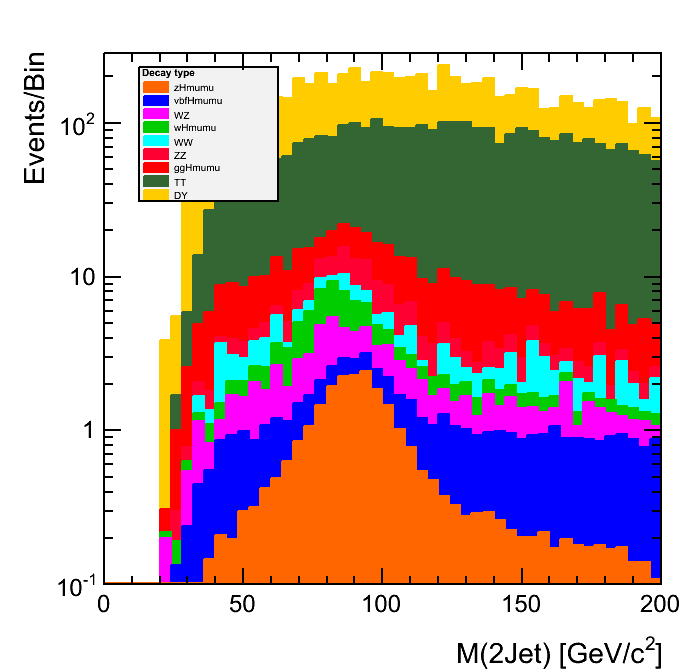
\includegraphics[width=0.49\textwidth]{images/Hist_jetMass.png}
    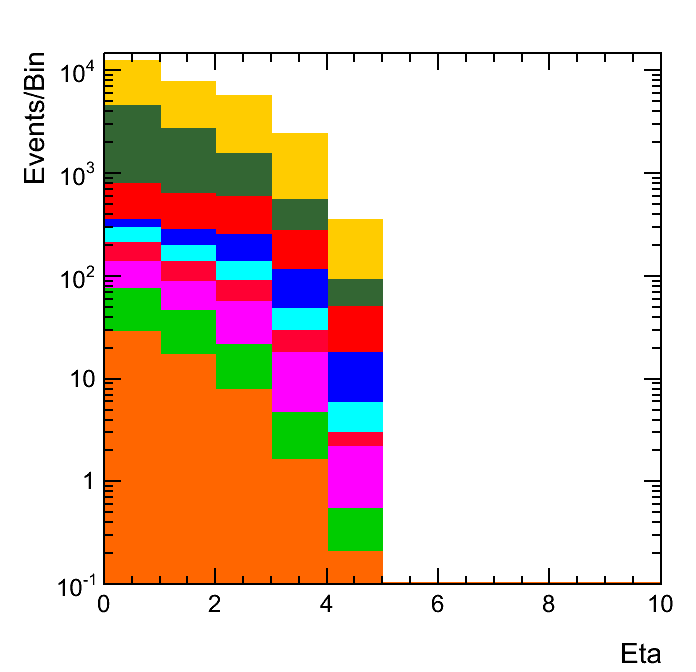
\includegraphics[width=0.49\textwidth]{images/Hist_jetEta.png}
    \caption{ \label{fig:Mjj}
         a) This plot shows the 2 Jet invariant mass after the preconditions have been applied. b) This plot shows the $\eta$
	 values after the Dimuon selection and Jet $p_{T}$ cut. The orange and light green events are the signal events and the other colors
	 are background.
      }
\end{center}
\end{figure}
For this criteria, we found that a lower limit of 60 GeV/c$^{2}$ and an upper limit of 110 GeV/c$^{2}$ were the best limits 
because they encompassed both the W peak and the Z peak. 
This cut has $\frac{S}{\sqrt{B}}$ = 1.24. For the rest of the selection criteria optimization we used only the following preconditions: 
the Dimuon selection, the Jet $p_{T}$ cut, the Jet $\eta$ cut, and the Dijet mass cut.

After optimizing our basic selection criteria and determining our preconditions, 
we optimized the selections on the transverse Angle Between the Higgs and vector boson ($\phi$), missing transverse Momentum and dimuon transverse momentum. 
We found an upper limit of -0.95 for the $cos$ of the transverse angle between the Higgs and vector boson to be the best (Figure \ref{fig:cosPhi}).
When combine all of the selection criteria, $\frac{S}{\sqrt{B}} $ = 1.82.
\begin{figure}[!hbtp]
\begin{center}
    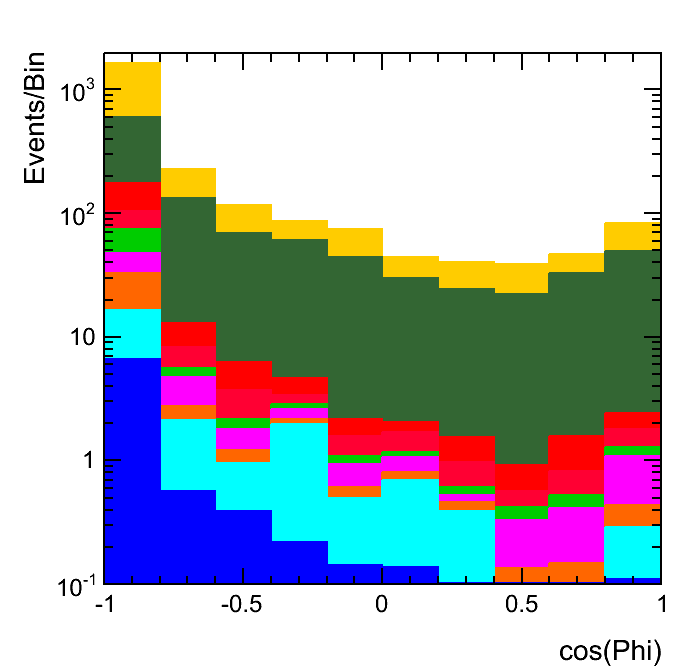
\includegraphics[width=0.49\textwidth]{images/Hist_MuMu2JetPhiBeforeCuts.png} %Redo this plot!!!!
    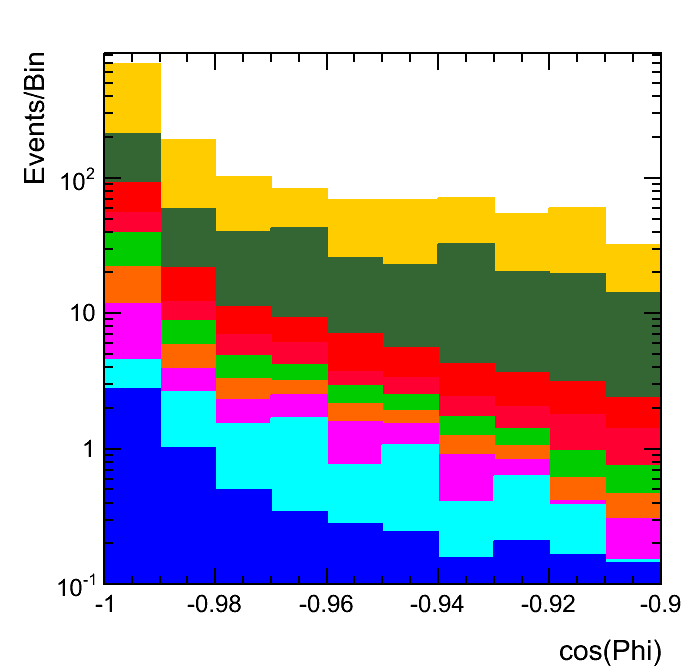
\includegraphics[width=0.49\textwidth]{images/Hist_MuMu2JetPhiZoomB4Cut.png}
    \caption{ \label{fig:cosPhi}
         a) This plot shows the $cos(\phi)$ value after the preconditions have been applied. b) This plot is a close-up of plot a.
	 The orange and light green events are the signal events and the rest others are background.
      }
\end{center}
\end{figure} 
This cut has $\frac{S}{\sqrt{B}}$ = 1.18. For the missing transverse momentum we found an upper limit of 40 GeV/c to be the best (Figure \ref{fig:ptmiss}a).
This cut has $\frac{S}{\sqrt{B}}$ = 1.12. Finally, we found a lower limit of 110 GeV/c to be the best for the dimuon transverse momentum selection 
(Figure \ref{fig:ptmiss}b). This cut has $\frac{S}{\sqrt{B}}$ = 1.20.
\begin{figure}[!hbtp]
\begin{center}
    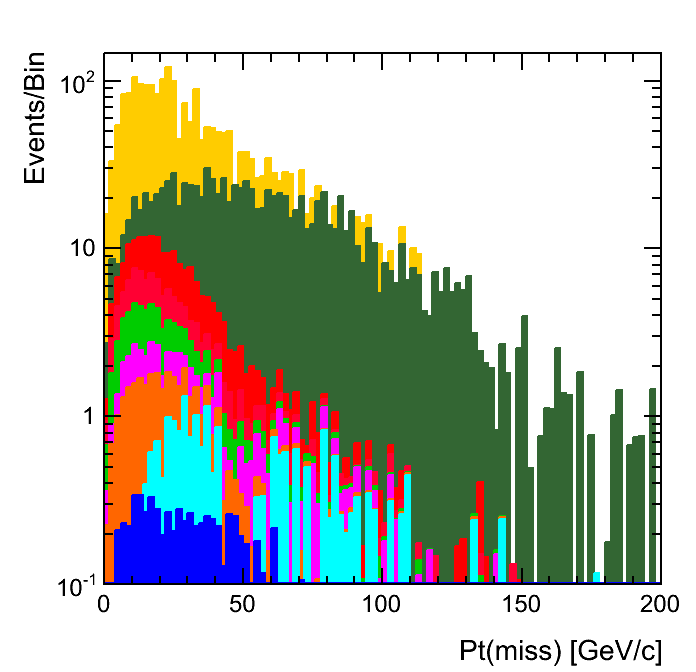
\includegraphics[width=0.49\textwidth]{images/Hist_PtMiss.png}
    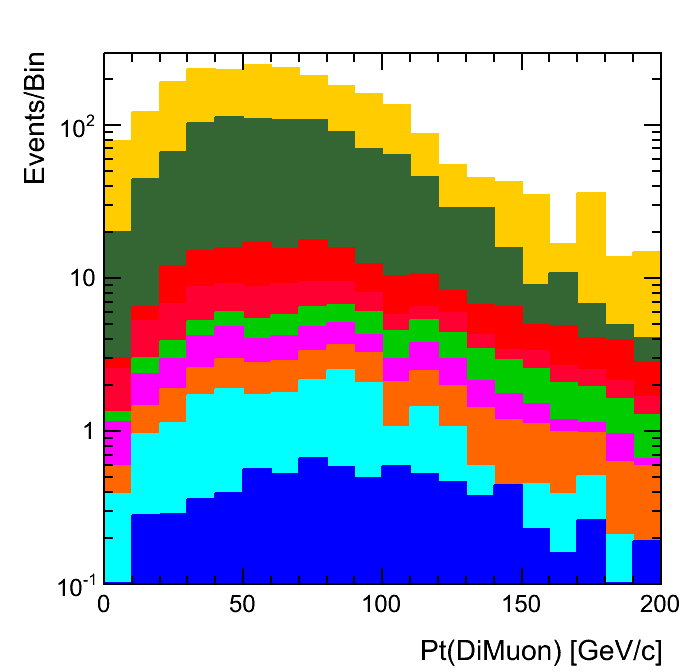
\includegraphics[width=0.49\textwidth]{images/Hist_DiMuonPt.png}
    \caption{ \label{fig:ptmiss}
         a) This plot shows the $p^{miss}_{T}$ values after the preconditions have been applied. b) This plot shows the dimuon $p_{T}$ values 
	 after the preconditions have been applied. The orange and light green events are the signal events and the rest others are background.
      }
\end{center}
\end{figure} 

%<Table with S/sqrtB ratio values>

\subsection{Choosing Correct Dijet}

In the VBF category, selection took place on the two highest $p_{T}$ jets. 
Similarly, we started off using the two highest $p_{T}$ jets for the VH category, 
but we soon discovered that some of the dijet combinations had unusually extreme values. 
Therefore, we decided to alter our selection criteria to see if we could pick up the correct jets. 
Instead of taking the highest $p_{T}$ jets, we selected for the highest dijet $p_{T}$ pair. This is shown 
in figure \ref{fig:dijetSel}. This improved our peak, but we still seem to be missing jets.
\begin{figure}[!hbtp]
\begin{center}
    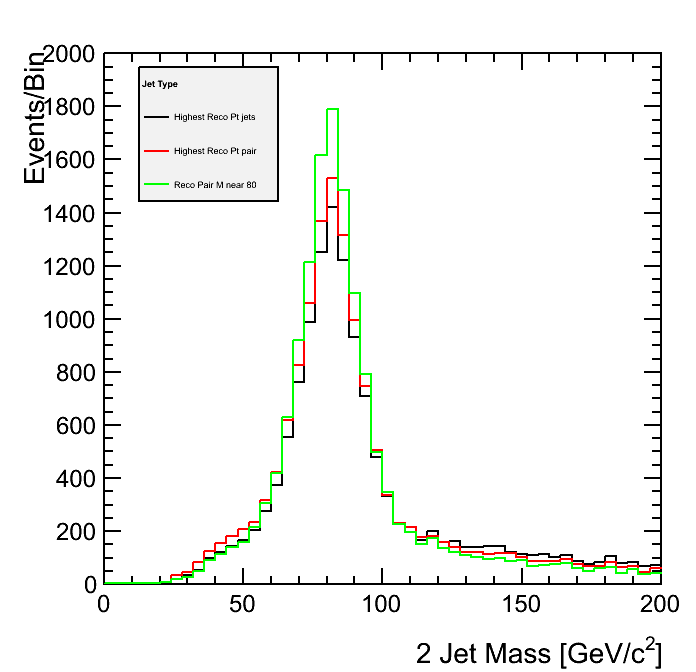
\includegraphics[width=0.49\textwidth]{images/Hist_Reco2PlotsPt30Eta2.png}
    \caption{ \label{fig:dijetSel}
         This shows the dijet pair selection in $WH$ for the event pair with a mass closest to 80 (a flawed selection that 
	 shows the best possible values), the event pair with the highest $p_{T}$, and the event pair created from the two highest $p_{T}$ jets.
      }
\end{center}
\end{figure}

\subsection{Maximum Likelihood Fits for Dijet Mass}

We explored the possibility of using a Maximum Likelihood fit to narrow the signal peak, but this technique did not yield any benefit.

\section{VH Analysis Optimization 2 (for 8 TeV data)}

\subsection{Introduction}

After obtaining optimum values for the selection criteria in the VH category, we applied these categories to the full 8 TeV analysis on real data. 
We then re-optimized the VH category based off of expected limits. 

\subsection{Expected Limits Definition}

Expected upper limits are computed using the asymptotic likelihood-ratio-based approach of 
Ref.~\cite{stats}.  This is done with the CMS Higgs group ``combine'' tool using binned
fits of parameterized signal and background shapes to the dimuon invariant mass 
($m_{\mu\mu}$) data.  The signal shape is parameterized
as the sum of two Gaussians, with parameters fixed to values fit to signal MC.
The background shape is a Breit--Wigner plus $1/m_{\mu\mu}^2$ term, both multiplied
by an exponential.  The Breit-Wigner mass and width are pre-fit to Z-peak data and fixed.
The expected limit is computed
using background shapes fit to 19.7\,fb$^{-1}$ of 8\,TeV data in each category,
and assuming no Higgs signal (they are background-only expected limits).  The upper
limits are presented in terms of the $\mathrm{CL_s}$ criterion~\cite{cls}, and are computed for 
a 95\% confidence level.  These expected limits include no systematic uncertainties.

\subsection{Selection Optimization}

The current analysis on 8 TeV data includes a un-optimized $VH$ category. This category requires (after dimuon selection) 
that the leading jet has $p_{T} >$ 40 GeV/c and that the sub-leading jet has $p_{T} >$ 30 GeV/c. In order for the new category to run
on the full analysis, without significant alterations to the analysis, the jet $p_{T}$ values cannot change. Using only expected limit comparisons for 
optimization, we found that a lower limit of 40 GeV/c for leading jet $p_{T}$, a lower limit of 30 GeV/c for sub-leading jet $p_{T}$, an upper 
limit of 40 GeV/c for $p_{T}^{miss}$, a lower limit of 110 GeV/c for dimuon $p_{T}$, and an upper limit of 2.7 for leading and sub-leading 
jet $|\eta|$ to have the best expected limit value at 92.5781. The expected limit values are shown in table \ref{tab:ExpectedLimits}.

\begin{table}[!hbtp]
  \begin{center}
    \caption{ \label{tab:ExpectedLimits}
        This Table is an optimization flow table of the $VH$ Category with preconditions of leading jet $p_{T} >$ 40
	GeV/c, sub-leading jet $p_{T} >$ 30 GeV/c, and $p_{T}^{miss} <$ 40 GeV/c.
    }
    \begin{tabular}{lcc} \hline \hline
         Selection Criteria & Expected limit \\ \hline
         60 GeV/c$^{2} < M_{jj} <$ 110 GeV/c$^{2}$ & 96.0938  \\
         + Dimuon $p_{T} >$ 110 GeV/c & 93.0469 \\
	 + Leading Jet $|\eta| <$ 2.7 & 93.0469 \\
	 + Sub-Leading Jet $|\eta| <$ 2.7 & 92.5781 \\
     \hline \hline
    \end{tabular}
  \end{center}
\end{table}

\section{VH Analysis Optimization 3 (for 13 TeV simulated data)}

\section{Background Fits involving Numeric Convolution}

\begin{thebibliography}{9}

\bibitem{AN2012_459}
  Acosta, D., et. al.,
  ``Search for standard model Higgs boson production in the $\mu^+\mu^-$ final state with the CMS experiment in pp collisions at $\sqrt{s}=7$ and 8\, TeV'',
  CMS Analysis Note AN-12459,
  2014.

\bibitem{PUID}
  CMS Collaboration, ``Pileup Jet Identification'', 
  CMS Physics Analysis Summary CMS-PAS-JME-13-005, 
  2013.

\bibitem{stats}
  ATLAS and CMS Collaborations, and LHC Higgs Combination Group, ``Procedure for
  the LHC Higgs boson search combination in summer 2011'', 
  CMS-NOTE-2011/005 ATL-PHYS-PUB-2011-011, 2011.

\bibitem{cls}
  A. L. Read, ``Presentation of search results: the CLs technique'', J. Phys. G 28 (2002) 2693,
  doi:10.1088/0954-3899/28/10/313.

\bibitem{pythia} 
  T.~Sjostrand, S.~Mrenna and P.~Z.~Skands,
  ``PYTHIA 6.4 Physics and Manual,''
  JHEP {\bf 0605}, 026 (2006)
  [hep-ph/0603175].

\bibitem{herwigpp} 
  M.~Bahr, S.~Gieseke, M.~A.~Gigg, D.~Grellscheid, K.~Hamilton, O.~Latunde-Dada, S.~Platzer and P.~Richardson {\it et al.},
  ``Herwig++ Physics and Manual,''
  Eur.\ Phys.\ J.\ C {\bf 58}, 639 (2008)
  [arXiv:0803.0883 [hep-ph]].

\bibitem{powheg1} 
  S.~Alioli, P.~Nason, C.~Oleari and E.~Re,
  ``A general framework for implementing NLO calculations in shower Monte Carlo programs: the POWHEG BOX,''
  JHEP {\bf 1006}, 043 (2010)
  [arXiv:1002.2581 [hep-ph]].
  %%CITATION = ARXIV:1002.2581;%%

\bibitem{powheg2} 
  S.~Alioli, P.~Nason, C.~Oleari and E.~Re,
  ``NLO Higgs boson production via gluon fusion matched with shower in POWHEG,''
  JHEP {\bf 0904}, 002 (2009)
  [arXiv:0812.0578 [hep-ph]].
  %%CITATION = ARXIV:0812.0578;%%

\bibitem{powheg3} 
  P.~Nason and C.~Oleari,
  ``NLO Higgs boson production via vector-boson fusion matched with shower in POWHEG,''
  JHEP {\bf 1002}, 037 (2010)
  [arXiv:0911.5299 [hep-ph]].
  %%CITATION = ARXIV:0911.5299;%%

\bibitem{hmumuPap} 
  CMS Collaboration [CMS Collaboration],
  ``Search for the standard model Higgs boson in the dimuon decay channel in pp collisions at sqrt(s)= 7 and 8 TeV,''
  CMS-PAS-HIG-13-007.
  %%CITATION = CMS-PAS-HIG-13-007;%%
  %11 citations counted in INSPIRE as of 03 Sep 2014

\end{thebibliography}

\end{document}
